\chapter{Multi-GPU Programming}


我們生活在一個資訊量指數級增長的時代。線上服務和社群媒體平台正竭盡全力維持這龐大的計算需求。此外,搜尋引擎必須不斷改進其索引能力,同時運用機器學習的功能來掌握數據的龐大規模。如前所述,GPU是許多這類資料導向應用程式的首選平台。
儘管GPU處理數據的速度明顯快於CPU,但單一GPU的運算能力仍有其限制。因此,使用多個GPU來加速應用程式是很常見的做法。由於ROCm最初是為超大規模運算而建立的,它也提供了優秀的多GPU支援功能。在本章中,我們將探討ROCm可用的常見多GPU程式設計方法。 

\section{HIP Device APIs}

在探討多GPU程式設計之前,我們必須先學習如何選擇特定的GPU。當使用單一GPU時,不需要明確指定device,因為\term{HIP} API預設會使用GPU 0。在\lstref{lst:hip_device_example} 中展示了一個HIP的範例,說明如何使用API在時脈最快的GPU上執行程式。

\term{hipGetDeviceCount} 通常是HIP應用程式中第一個被呼叫的需要特定GPU的API。這個API會回傳可用的GPU數量。下一步是使用\term{hipGetDeviceProperties} 來查詢device屬性(例如:型號、主記憶體大小、核心時脈頻率和並行核心支援)。完整的可用屬性清單可以在\term{hipDeviceProp\_t} 結構中找到。

\begin{lstlisting}[language=C, caption={用時脈最快的GPU執行程式}, captionpos=t, label={lst:hip_device_example}]
int main() {
    int device_count;
    hipDeviceProp_t props;

    // Get GPU Count.
    hipGetDeviceCount(&device_count);

    // Find the GPU with the highest clock frequency.
    int fastest_gpu = 0;
    int fastest_gpu_freq = 0;
    for (int i = 0; i < device_count; i++) {
        hipGetDeviceProperties(&props, i);

        if (props.clockRate > fastest_gpu_freq) {
            fastest_gpu_freq = props.clockRate;
            fastest_gpu = i;
        }
    }
    printf("Fastest GPU: %d (%d KHz)\n",
        fastest_gpu, fastest_gpu_freq);

    // Select the GPU.
    hipSetDevice(fastest_gpu);

    // Allocate buffers, copy data, & launch kernel.

    return 0;
}
\end{lstlisting}

\term{hipSetDevice} 通過傳入一個整數參數來明確選擇特定的GPU或群組。之後,在同一執行緒上運行的API呼叫將使用相同的GPU,除非被更改。核心可以在這個GPU上啟動,而device同步API可以確保所有任務在返回前都已完成。請記住,\term{hipMalloc} 負責分配GPU記憶體。

要切換到另一個GPU,需要再次呼叫\term{hipSetDevice},且當前GPU的索引會被儲存為執行緒的本地變數。如果程式需要知道目前正在使用哪個device,\term{HIP} API提供了\term{hipGetDevice} 來查詢所選擇的device索引。在呼叫\term{hipSetDevice} 之前呼叫\term{hipGetDevice} 會回傳預設的GPU ID。此外,由於device索引是執行緒本地的,設定device不會影響其他執行緒所調用的API。

多GPU運算通過允許多個GPU參與適當的執行來提升GPU系統效能。在高層面上,我們必須控制GPU並平行分派任務。\term{ROCm}和\term{HIP}在CPU端提供了幾種平行任務分派的選項。第一個選項是使用串流,因為它們的任務可以平行執行。因此,我們為每個GPU創建一個CPU執行緒,每個執行緒控制一個GPU。最後,如果手動創建和同步執行緒過於複雜,可以使用MPI相關的函式庫來顯著降低複雜度。因此,在接下來的三個章節中,我們將介紹三種多GPU程式設計方案:基於串流(stream)、執行緒(thread)和MPI的方法。

請注意,上述方法的效能通常是相當的,選擇哪種方法通常取決於程式設計師的偏好和判斷,這要視問題的類型而定。值得注意的是,這些方法可以結合使用,例如使用兩個CPU執行緒來控制四個GPU,並在這兩個CPU執行緒中各自使用基於串流的方法。這讓程式設計師能夠靈活地編寫富有表現力且易於管理的多GPU程式。

\section{Stream-Based Muiti-GPU Programming}

在不同串流中排隊的任務可以平行執行。利用這個特性,使用串流是最簡單的平行GPU程式設計方法。在執行任何GPU相關任務之前,會為每個GPU創建一個串流。然後,在每個queue中啟動核心,通常是以迴圈的形式,因為我們很可能會在多個GPU上啟動相同的核心。由於核心啟動是非同步的,程式可以在啟動其他核心的同時執行下一個迭代,而無需等待當前核心完成。最後,我們以同步方式等待所有核心完成。

一個使用多個GPU執行\term{vector\_add}運算的簡單範例在\lstref{lst:multiGPUs_streams} 
 中展示。注意,有三個分別遍歷GPU的獨立迴圈。第一個迴圈創建queue、分配記憶體並將記憶體複製到GPU。第二個迴圈啟動核心。最後,第三個迴圈作為同步障礙(barrier),確保所有核心在正確的時間完成執行。第一和第二個迴圈中的第一行呼叫\term{hipSetDevice},用於選擇每次迭代要使用的GPU。在第三個迴圈中不需要再次呼叫\term{hipSetDevice},因為串流已經與所需的device關聯。

\begin{lstlisting}[language=C, caption={用stream設計多GPU程式}, captionpos=t, label={lst:multiGPUs_streams}]
int main() {
    int device_count;
    hipDeviceProp_t props;
    uint64_t length = 1024000000;
    int block_size = 256;
    int num_gpus = 8;
    int length_per_gpu = length / num_gpus;
    int num_block_per_gpu = (length_per_gpu - 1) / block_size + 1;

    std::vector<float> a, b, c;
    for (int i = 0; i < length; i++) {
        a.push_back((float)rand() / (float)RAND_MAX);
        b.push_back((float)rand() / (float)RAND_MAX);
    }

    std::vector<float*> d_a, d_b, d_c;
    std::vector<hipStream_t> streams;

    for (int i = 0; i < num_gpus; i++) {
        hipSetDevice(i);

        hipStream_t stream;
        hipStreamCreate(&stream);
        streams.push_back(stream);

        float *a_ptr, *b_ptr, *c_ptr;
        hipMalloc((void**)&a_ptr,
            length_per_gpu * sizeof(float));
        hipMalloc((void**)&b_ptr,
            length_per_gpu * sizeof(float));
        hipMalloc((void**)&c_ptr,
            length_per_gpu * sizeof(float));

        d_a.push_back(a_ptr);
        d_b.push_back(b_ptr);
        d_c.push_back(c_ptr);

        hipMemcpy(a_ptr,
            a.data() + i * length_per_gpu,
            length_per_gpu * sizeof(float),
            hipMemcpyHostToDevice);
        hipMemcpy(b_ptr,
            b.data() + i * length_per_gpu,
            length_per_gpu * sizeof(float),
            hipMemcpyHostToDevice);
    }

    for (int i = 0; i < num_gpus; i++) {
        hipSetDevice(i);
        vec_add<<<num_block_per_gpu, block_size, 0, streams[i]>>>(
            d_a[i], d_b[i], d_c[i], length_per_gpu);
    }

    for (int i = 0; i < num_gpus; i++) {
        hipStreamSynchronize(streams[i]);
    }

    c.resize(length);
    for (int i = 0; i < num_gpus; i++) {
        hipSetDevice(i);
        hipMemcpy(c.data() + i * length_per_gpu,
            d_c[i],
            length_per_gpu * sizeof(float),
            hipMemcpyDeviceToHost);
    }

    // Use the result and free the GPU memory.

    return 0;
}
\end{lstlisting}

當所有GPU執行相同的核心,且程式需要頻繁同步時,基於stream的多GPU程式設計方式相當便利。然而,在某些應用中,GPU可能需要處理不同的任務,且只需要有限的同步。在這種情況下,使用基於stream的方法來實現這些需求可能會使程式變得冗長且難以管理。我們希望每個GPU都能有自己獨立的任務流程(例如:記憶體複製和核心啟動),並且只在必要時進行同步。為了簡化這種目的的程式設計,接下來我們將介紹基於執行緒的多GPU程式設計。

\section{Thread-Based Multi-GPU Programming}

基於執行緒的多GPU程式設計相當直觀。我們首先為每個GPU創建並啟動一個執行緒,每個執行緒呼叫\term{hipSetDevice} 來綁定特定的GPU。然後,我們可以呼叫其他\term{HIP} API來控制GPU。
通常,大多數基於執行緒的多GPU程式設計需要同步。然而,這可以使用常規的C/C++執行緒同步原語來完成(例如:joins、mutexes和條件變數)。因此,我們不會深入探討這個主題。

在 \lstref{lst:multGPUs_threads} 中,我們提供了相同的多GPU \term{vector\_add}範例,但使用基於執行緒的方法來實現。這次,我們指定一個從名為\bold{gpu\_thread}的函式開始的CPU執行緒來執行GPU相關任務。該函式將GPU ID作為參數,這樣它就能與特定GPU建立關聯,並在函式的第一行程式碼中進行綁定。執行緒函式的其餘部分就像單GPU程式碼一樣運作。

由於我們將所有GPU任務都委託給了執行緒,main函式除了宣告和初始化數據外,不需要進行其他\term{HIP} API呼叫。在main函式中只需要啟動一組執行緒,每個GPU一個,並將它們全部同步。在這個範例中,我們使用\term{join}函式來等待所有執行緒結束。

\begin{lstlisting}[language=C, caption={用執行緒設計多GPU程式}, captionpos=t, label={lst:multGPUs_threads}]
void gpu_thread(int gpu_id, int length_per_gpu, float* A, float* B, float* C) {
    hipSetDevice(gpu_id);
    
    printf("gpu_thread %d\n", gpu_id);
    
    int n = length_per_gpu;
    
    float *dA, *dB, *dC;
    hipMalloc(&dA, n * sizeof(float));
    hipMalloc(&dB, n * sizeof(float));
    hipMalloc(&dC, n * sizeof(float));
    
    hipMemcpy(dA, A, n * sizeof(float), hipMemcpyHostToDevice);
    hipMemcpy(dB, B, n * sizeof(float), hipMemcpyHostToDevice);
    
    int block_size = 256;
    int grid_size = (n + block_size - 1) / block_size;
    vec_add<<<grid_size, block_size>>>(dA, dB, dC, n);
    
    hipMemcpy(C, dC, n * sizeof(float), hipMemcpyDeviceToHost);
    
    hipDeviceSynchronize();
    
    hipFree(dA);
    hipFree(dB);
    hipFree(dC);
}

int main() {
    hipError_t err;
    int device_count;
    hipDeviceProp_t props;
    
    uint64_t length = 102400;
    int num_gpus = 8;
    int length_per_gpu = length / num_gpus;
    if (length % num_gpus != 0) {
        fprintf(stderr, "length must be a multiple of num_gpus\n");
        return 1;
    }
    
    std::vector<float> a, b, c;
    for (int i = 0; i < length; i++) {
        a.push_back((float)rand() / (float)RAND_MAX);
        b.push_back((float)rand() / (float)RAND_MAX);
    }
    c.resize(length);
    
    std::vector<std::thread> threads;
    for (int i = 0; i < num_gpus; i++) {
        threads.push_back(std::thread(
            gpu_thread, i, length_per_gpu, a.data() + i * length_per_gpu,
            b.data() + i * length_per_gpu, c.data() + i * length_per_gpu));
    }
    
    for (int i = 0; i < num_gpus; i++) {
        threads[i].join();
    }
    
    // Use the result.
    
    return 0;
}
\end{lstlisting}

\section{MPI-Based Multi-GPU Programming}

\term{MPI} 通訊標準在高效能多核心和分散式運算環境中被廣泛使用。它最初是為了管理大量CPU執行緒而設計,能自動啟動執行相似任務的執行緒,包括允許不同執行緒共享資料的通訊原語。由於\term{MPI} 標準在HPC社群中的普及性,\term{HIP} 支援基於\term{MPI} 的多GPU運算,這與執行緒基礎的方法非常相似。唯一的區別在於\term{MPI} 負責處理執行緒的建立、通訊和同步化,這減少了程式設計師在管理執行緒時的負擔。

我們使用\term{MPI} 來控制多個GPU展示一個簡單的範例(參見\lstref{lst:multGPUs_mpi})。我們建立一個隨機陣列(第25行),將其分散到各個GPU(第36行),計算每個元素的平方(第49行),將結果收集回根GPU(第60行),並對平方元素進行求和(第72行)。

此範例中有幾行程式碼是\term{MPI} 專用的。在主程式開始時,我們首先通過呼叫 \term{MPI\_Init(\&argc, \&argv)} 來初始化\term{MPI} 環境。在此範例中,我們假設處理程序的數量等於使用的GPU數量。請注意,\term{MPI} 也允許使用者在每個GPU上執行多個\term{MPI} 處理程序,但我們在此並未使用此功能。接下來,我們使用\term{MPI\_Comm\_rank} 和\term{MPI\_Comm\_size} 分別獲取當前rank編號和rank總數。編號和計數提供了必要的位置資訊,使每個處理程序都知道要處理的資料部分。通訊rank編號也可用於將處理程序與其對應的GPU關聯起來。在此範例中,我們假設處理程序的rank ID等於其所控制的GPU的ID。

在程式的主體部分,我們使用多個\term{MPI} 通訊原語,包括\term{MPI\_Scatter} 和\term{MPI\_Gather} 。它們支援CPU緩衝區之間的資料傳輸,而不是GPU-GPU通訊。這種實作方式並非最有效的解決方案,因為涉及了額外(且不必要)的CPU-GPU資料移動。例如,在第51行,我們將平方結果複製到等級本地緩衝區,這樣在第60行收集資料後,我們可以在第67行將結果複製回GPU。理想情況下,如果我們能直接在GPU記憶體中匯總資料,就能避免這些額外的記憶體複製。為了實現直接的GPU-GPU資料匯總,我們接下來介紹\term{ROCM} 的點對點通訊功能(見 \autoref{sec:10.5})和\term{RCCL} (見 \autoref{sec:10.6})。

\begin{lstlisting}[language=C, caption={用MPI設計多GPU程式}, captionpos=t, label={lst:multGPUs_mpi}]
// square kernel implementation is neglected
// reduction_sum implementation is neglected
// create_rand_nums implementation is neglected

int main(int argc, char** argv) {
    // Initialize the MPI environment
    MPI_Init(&argc, &argv);
    
    // Find out rank, size
    int world_rank, world_size;
    MPI_Comm_rank(MPI_COMM_WORLD, &world_rank);
    MPI_Comm_size(MPI_COMM_WORLD, &world_size);
    
    int num_elements_per_proc = atoi(argv[1]);
    int total_elements = world_size * num_elements_per_proc;
    int data_in_bytes_per_node = num_elements_per_proc * sizeof(int);
    int total_data_in_bytes = total_elements * sizeof(int);

    
    // Create a random array of elements on the root process.
    srand(time(NULL));
    int *rand_nums = NULL;
    if (world_rank == 0) {
        rand_nums = create_rand_nums(total_elements);
    }
    
    // For each process, create a buffer that will hold a subset of the
    // array
    int *sub_rand_nums = (int *)malloc(data_in_bytes_per_node);
    int *results = (int *)malloc(data_in_bytes_per_node);

    
    // Scatter the random numbers from the root process to all processes in
    // the MPI world.
    MPI_Scatter(rand_nums, num_elements_per_proc, MPI_INT, sub_rand_nums,
                num_elements_per_proc, MPI_INT, 0, MPI_COMM_WORLD);

    hipSetDevice(world_rank);
    
    int *d_sub_rand_nums, *d_results;
    hipMalloc(&d_sub_rand_nums, data_in_bytes_per_node);
    hipMalloc(&d_results, data_in_bytes_per_node);
    hipMemcpy(d_sub_rand_nums, sub_rand_nums, data_in_bytes_per_node, hipMemcpyHostToDevice);
              
    int blockSize, gridSize;
    blockSize = 32;
    gridSize = (int)ceil((float)num_elements_per_proc/blockSize);
    square<<<gridSize, blockSize>>>(d_sub_rand_nums, d_results, num_elements_per_proc);                 
    hipDeviceSynchronize();
    hipMemcpy(results, d_results, data_in_bytes_per_node, hipMemcpyDeviceToHost);
              
    int *aggregated_results = NULL;
    if (world_rank == 0) {
        aggregated_results = (int *)malloc(total_data_in_bytes);
    }
    
    MPI_Barrier(MPI_COMM_WORLD);
    
    MPI_Gather(results, num_elements_per_proc, MPI_INT, aggregated_results, num_elements_per_proc, MPI_INT, 0, MPI_COMM_WORLD);



    if(world_rank == 0) { // Root node to gather the data.
        int *d_aggregated_results = NULL;
        hipMalloc(&d_aggregated_results, total_data_in_bytes);
        hipMemcpy(d_aggregated_results, aggregated_results, total_data_in_bytes, hipMemcpyHostToDevice);
        
        int *d_output;
        hipMalloc(&d_output, sizeof(int));
        
        reduction_sum(d_aggregated_results, d_output, total_elements);
        
        int reduce_sum = 0;
        hipMemcpy(&reduce_sum, d_output, sizeof(int), hipMemcpyDeviceToHost);
        printf("Reduce sum %d\n", reduce_sum);
    }
    
    MPI_Finalize();
    
    // Free CPU and GPU memory buffers.
}
\end{lstlisting}

編譯和執行這個程式需要一些特殊的命令。假設\term{MPI} 函式庫已經正確安裝,第一個命令是\bold{mpicc --showme}。編譯器\term{mpicc} 是\bold{gcc}命令的包裝器(wrapper),但包含了\term{MPI} 相關檔案和預定義連結的特殊參數。\bold{--showme}參數會顯示當使用\bold{gcc}時的等效命令。在我們的平台上,該命令的輸出如下:

\begin{lstlisting}[numbers=none, caption={\bold{mpicc --showme}的輸出}, captionpos=t, label={lst:output_of_mpiccshowme}]
gcc
    -I/usr/lib/x86_64-linux-gnu/openmpi/include/openmpi
    -I/usr/lib/x86_64-linux-gnu/openmpi/include/openmpi/opal/mca/event/libevent2022/libevent
    -I/usr/lib/x86_64-linux-gnu/openmpi/include/openmpi/opal/mca/event/libevent2022/libevent/include
    -I/usr/lib/x86_64-linux-gnu/openmpi/include
    -pthread
    -L/usr/lib
    -L/usr/lib/x86_64-linux-gnu/openmpi/lib
    -lmpi
\end{lstlisting}

要編譯具有\term{MPI} 支援的\term{HIP} 程式,我們必須將\term{gcc}替換為\term{hipcc}。然後,\term{MPI} 函式庫將會被連結到編譯後的執行檔。
要運行編譯後的程式,使用\bold{mpirun}命令。行程數量(也就是GPU的數量)是由\bold{mpirun}命令提供的。假設我們想要使用四個GPU,且編譯後的程式名為main,我們使用\bold{mpirun -n 4 ./main}來執行程式。

\begin{figure}[h]
    \centering
    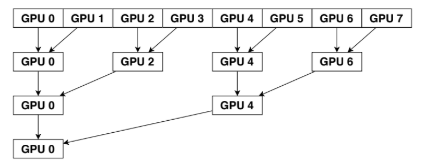
\includegraphics[width=0.75\linewidth]{FileAusiliari//Screenshots/Figure10-1.png}
    \caption{GPU-level 歸約}
    \label{fig:gpu-level-reduction}
\end{figure}

\section{GPU-GPU Communication} \label{sec:10.5}

在先前展示的範例中,CPU負責將數據分配給GPU,然後由GPU進行處理。然而,在許多情況下,GPU之間需要相互通訊。例如,一個常見的多GPU計算模式允許每個GPU對不同的輸入數據獨立執行相同的運算,並在本地儲存輸出結果。然後我們對這些輸出進行匯總(例如:平均或求和)以得到最終結果。雖然第一階段中每個GPU的獨立計算不需要GPU之間的通訊,但第二階段(匯總)則需要。如\term{MPI} 範例中所討論的,將數據複製回CPU進行匯總是低效的。

通常,匯總數據的情況需要一個GPU版的歸約演算法,如 \autoref{fig:gpu-level-reduction} 所示。如果數據分佈在八個GPU上,歸約需要三次迭代($log_{2}8$ = 3)。在每次迭代中,數據會在兩個GPU之間進行匯總。因此,每次迭代中活躍的GPU數量會減半。在本節的其餘部分,我們使用一個歸約演算法來展示GPU-GPU通訊。具體來說,我們對儲存在八個GPU上的數據求平均值,並將最終結果儲存在GPU 0的輸入緩衝區中。

使用\term{HIP} 時,我們有兩種GPU-GPU通訊選項:常規記憶體複製或點對點通訊。\term{HIP} 提供了必要的API。一般的\term{hipMemcpy} 指定了複製方向,如\term{hipMemcpyDeviceToDevice}。為了便利,\term{HIP} 還提供了一個專門的API:\term{hipMemcpyDtoD},用於設備間的記憶體複製。

我們在 \lstref{lst:dtd_mutiGPUs} 中實現了一個八個GPU歸約的範例。對於每個匯總步驟,我們首先在GPU上創建緩衝區。例如,對於GPU 0和1,我們在GPU 0上創建一個緩衝區。然後我們使用\term{hipMemcpyDtoD} 將數據從GPU 1複製到GPU 0上新創建的緩衝區。最後,我們在GPU 0上啟動平均值核心來匯總數據。該核心完全在本地數據上操作,在核心運行時不需要GPU間通訊。

\begin{lstlisting}[language=C, caption={用device-to-device記憶體複製達到多GPU溝通}, captionpos=t, label={lst:dtd_mutiGPUs}]
int main() {
    uint64_t length = 1024;
    int num_gpu = 8;
    std::vector<std::vector<float>> h_output(num_gpu);
    std::vector<float*> output_gpu(num_gpu);
    float* final_result;
    
    // Stage 1, calculate the result for otuput_gpu buffers.
    for (int i = 0; i < num_gpu; i++) {
        // Neglected
    }

    for (int i = 1; i < num_gpu; i = i << 1) {
        for (int j = 0; j < num_gpu; j += (i * 2)) {
            int leftGPU = j;
            int rightGPU = j + i;
            printf("Calculating average between GPU %d and %d\n", leftGPU,
                    rightGPU);
            
            hipSetDevice(leftGPU);
            
            float* leftBuf = output_gpu[leftGPU];
            float* rightBuf;
            hipMalloc(&rightBuf, (size_t)length * sizeof(float));
            hipMemcpyDtoD(rightBuf, output_gpu[rightGPU],
                         (size_t)length * sizeof(float));
            
            int block_size = 256;
            int num_block = (length - 1) / block_size + 1;
            avg<<<num_block, block_size>>>(leftBuf, rightBuf, length);
        }
    }
    
    // Use final_result.
    return 0;
}
\end{lstlisting}

基於記憶體複製的GPU-GPU通訊是一個簡單但有效的解決方案。它能以可預測的效能將數據從一個GPU移動到另一個GPU。當複製大量數據時,\term{ROCm}經過優化可以充分利用GPU之間的頻寬。因此,這種方法適合一般用途。唯一的問題是,在所有數據到達之前,計算核心無法開始執行,因此錯過了重疊數據移動和計算的機會。

點對點通訊解決方案允許程式設計師更細緻地控制通訊和計算。在高層面上,GPU核心可以輕鬆訪問另一個GPU上的實體定位記憶體,而無需核心修改,從而實現點對點通訊。只需將指標作為核心參數傳遞到遠程地址即可。這些機制由\term{ROCm}在AMD GPU上提供,對程式設計師來說是完全透明的。

在 \lstref{lst:ptp_multiGPUs} 中,我們使用點對點通訊重新實現相同的八個GPU平均值範例。大部分程式碼(包括計算平均值的核心)保持不變。然而,這裡有幾個值得注意的要點。首先,在使用這個功能之前,我們必須檢查我們的平台是否支援點對點通訊。這可以通過呼叫\term{hipDeviceCanAccessPeer} 來完成。如果不支援,我們可以回到基於記憶體複製的解決方案或使用CPU記憶體作為中間緩衝區。其次,點對點通訊預設是不啟用的;因此,需要使用\term{hipDeviceEnablePeerAccess} 手動啟用此功能。請注意,啟用點對點訪問在某些情況下可能會降低GPU效能,當不需要此功能時,應使用\term{hipDeviceDisablePeerAccess} 或\term{hipDeviceReset} 關閉它。

當使用點對點通訊功能時,我們可以跳過創建複製數據的中間緩衝區這個步驟。在這個範例中,點對點記憶體複製減少了程式設計的複雜性。

\begin{lstlisting}[language=C, caption={用點對點存取達到多GPU溝通}, captionpos=t, label={lst:ptp_multiGPUs}]
// Calculate the element-wise average of A and B
// and store the result back in A.
__global__ void avg(float* A, float* B, int n) {
    // Content of the kernel neglected for brevity.
}

int main() {
    uint64_t length = 1024;
    int num_gpu = 8;
    std::vector<std::vector<float>> h_output(num_gpu);
    std::vector<float*> output_gpu(num_gpu);
    float* final_result;
    
    // Stage 1, calculate the results to store in the output_gpu buffers.
    for (int i = 0; i < num_gpu; i++) {
        // Neglected
    }
    
    for (int i = 1; i < num_gpu; i = i << 1) {
        for (int j = 0; j < num_gpu; j += (i * 2)) {
            int leftGPU = j;
            int rightGPU = j + i;
            printf("Calculating average between GPU %d and %d\n", leftGPU, 
                   rightGPU);
            
            // Check if peer-to-peer memory access is enabled.
            int canAccessPeer = 0;
            err = hipDeviceCanAccessPeer(
                &canAccessPeer, left_gpu, right_gpu);
            if (err != hipSuccess) {
                fprintf(stderr, "Can't access peer device %d\n", right_gpu);
                exit(EXIT_FAILURE);
            }
            printf("Can access peer %d\n", canAccessPeer);
            
            // Enable peer-to-peer memory access.
            hipSetDevice(leftGPU);
            err = hipDeviceEnablePeerAccess(right_gpu, 0);
            if (err != hipSuccess) {
                fprintf(stderr, "Can't enable peer access to device %d\n", 
                       right_gpu);
                exit(EXIT_FAILURE);
            }
            
            // We do the memory copy next.
            float* leftBuf = output_gpu[leftGPU];
            float* rightBuf = output_gpu[rightGPU];
            
            int block_size = 256;
            int num_block = (length - 1) / block_size + 1;
            avg<<<num_block, block_size>>>(leftBuf, rightBuf, length);
        }
    }
    
    // Use final_result.
    return 0;
}
\end{lstlisting}

點對點方法的效能影響是可以很複雜的。比如,\term{avg}核心直接對遠程GPU發出記憶體存取請求,因此GPU在一小塊資料到達後就可以進行計算,不需要等待整個緩衝區完成複製。此外,較長的GPU-GPU通訊延遲可能會對整體效能產生負面影響。最後,GPU之間的頻寬可能無法被充分利用。如果程式設計師不具備關於點對點操作的深入知識或未進行效能調校,他們應該謹慎使用點對點記憶體存取功能。

\section{RCCL}

在前一節介紹的範例中,我們討論了如何匯總在不同GPU上的數據。考慮到此類操作的潛在需求,\term{ROCm} 提供了使用\term{RCCL} 來大幅簡化數據分配和協作的能力,這是專為AMD GPU平台預先優化的;因此程式設計師通常可以期待比自己實現更高的效能。\term{RCCL} 是GPU版本的\term{MPI} 基本功能,而且它避免了在先前\term{MPI} 範例中提到的額外記憶體複製。

\term{RCCL} 遵循NVIDIA的集體通訊函式庫(\term{NCCL})API。因此,大多數\term{RCCL} API都帶有"nccl"前綴。如果現有應用程式是用\term{NCCL} 編寫的,就只需要最少的修改。

\term{RCCL} 支援一系列通訊基本功能,包括\term{Broadcast}、\term{Reduce}、\term{All Reduce}、\term{All Gather}和\term{Reduce Scatter}。我們提供兩個展示\term{RCCL} 功能的範例,一個使用\term{Broadcast},另一個使用\term{AllReduce}。像其他多GPU程式設計函式庫一樣,\term{RCCL可}以以串流、執行緒或基於\term{MPI}的方式使用。我們在\term{Broadcast}範例中展示基於串流的\term{RCCL}呼叫,在\term{AllReduce}範例中展示基於\term{MPI}的\term{RCCL}呼叫。雖然我們只展示了\term{Broadcast}和\term{AllReduce}範例,但讀者會發現其他基本功能的語法也很相似。

\subsection{Broadcast}

\term{Broadcast} 是最簡單的\term{RCCL} 基本功能。如 \autoref{fig:RCCL_Broadcast_primitive} 所示,它將數據項從單一GPU發送到多個GPU。\lstref{lst:mpi_rccl_broadcast} 提供了使用\term{Broadcast} 的範例。在這個範例的開始,我們包含了兩個標頭檔:常規的\term{hip\_runtime.h} 和\term{rccl.h}。\term{hip\_runtime.h} 用於其記憶體、device和串流管理功能。

\begin{figure}[h]
    \centering
    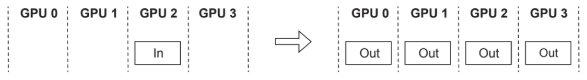
\includegraphics[width=0.75\linewidth]{FileAusiliari//Screenshots/Figure10-2.png}
    \caption{RCCL Broadcast 基本功能}
    \label{fig:RCCL_Broadcast_primitive}
\end{figure}

在\term{RCCL} 通訊過程開始之前,我們必須使用\term{hipMalloc} 創建一個緩衝區列表。每個GPU都分配一個緩衝區,而源緩衝區(GPU 0)則填入預定義的數據以廣播到所有其他GPU。在這個範例中,我們為每個GPU創建一個單一緩衝區。對於廣播根(GPU 0),源緩衝區與目標緩衝區相同;因此,不需要在源GPU上執行數據複製。然而,\term{RCCL Broadcast} 基本功能支援複製到一組與源不同的緩衝區。

啟動\term{RCCL} 數據傳輸的第一步是創建一個通訊器列表。通常每個GPU創建一個通訊器,而\term{RCCL} 提供了一個方便的API(\term{ncclCommInitAll}),可以一次初始化多個通訊器。由於使用多個通訊器可能會導致死鎖,我們必須謹慎設計同步策略;因此,不建議為一個GPU使用多個通訊器。

使用\term{ncclBroadcast} 完成廣播操作。由於我們要將數據廣播到四個GPU(包括源GPU),因此API必須在迴圈中被調用四次,從第32行開始。

為了向\term{RCCL} 函式庫表明這四個API調用屬於同一個廣播操作,我們在\term{ncclBroadcast} 之前調用\term{ncclGroupStart},之後調用\term{ncclGroupEnd}。獨立的\term{RCCL}調用是為基於執行緒的多GPU程式設計而設計的。如果沒有\term{ncclGroupStart}調用,\term{RCCL} 會等待所有執行緒調用廣播API。在單執行緒環境中,這會在第一個\term{Broadcast} 調用時造成死鎖。這些API通知\term{RCCL} 它們將被作為單一執行緒調用,然後返回而不執行。實際執行僅在調用\term{ncclGroupEnd} 時發生。

\term{ncclBroadcast} 調用是非同步的。因此,我們傳入一個串流,API會將任務添加到串流中執行。在第41行,所有串流都同步以確保所有GPU都收到數據。

\begin{lstlisting}[language=C, caption={混合使用\term{MPI} 和\term{RCCL Broadcast}}, captionpos=t, label={lst:mpi_rccl_broadcast}]
#include <hip/hip_runtime.h>
#include <rccl.h>


int main(int argc, char* argv[]) {
    const int nDev = 4;
    int size = 1 * 1024;
    int devs[4] = {0, 1, 2, 3};
    std::vector<float> in(size);
    int root = 0;

    // Initialize input.

    // Allocating and initializing device buffers.
    float** buff = (float**)malloc(nDev * sizeof(float*));
    hipStream_t* s = (hipStream_t*)malloc(sizeof(hipStream_t) * nDev);

    for (int i = 0; i < nDev; ++i) {
        hipSetDevice(i);
        hipMalloc(buff + i, size * sizeof(float));
        hipStreamCreate(s + i);
    }

    hipSetDevice(root);
    hipMemcpyHtoD(buff[root], in.data(), size * sizeof(float));
    
    // Initialize
    ncclComm_t comms[nDev];
    ncclCommInitAll(comms, nDev, devs);
    
    ncclGroupStart();
    for (int i = 0; i < nDev; ++i) {
        ncclBroadcast((const void*)buff[i], (void*)buff[i], size,
                     ncclFloat, root, comms[i], s[i]);
    }
    ncclGroupEnd();
    
    // Wait for broadcast to complete.
    for (int i = 0; i < nDev; ++i) {
        hipSetDevice(i);
        hipStreamSynchronize(s[i]);
    }
    // Free allocated CPU and GPU memory buffers.
    return 0;
}
\end{lstlisting}

\subsection{AllReduce}

\term{AllReduce} 是另一個常見的\term{RCCL} 基本功能。如 \autoref{fig:RCCL_Allreduce_primitive} 所示,\term{AllReduce} 會匯總儲存在多個GPU上的數據並將其分發給所有其他GPU。

我們的\term{AllReduce} 使用案例涉及數據並行的多GPU DNN訓練,這通常始於將各種訓練數據分散到多個GPU上。然後每個GPU應用前向和後向傳播演算法來計算其梯度(即神經網路參數應該如何更新)。因為每個GPU使用不同的訓練數據,梯度也可能不同。\term{AllReduce} 用於對梯度取平均並將其分發給每個GPU。在所有GPU收到平均梯度後,它們更新各自本地儲存的DNN模型。在DNN模型更新後,GPU就可以接收另一批訓練數據。

在 \lstref{lst:mpi_rccl_allreduce} 的範例中,我們將\term{RCCL AllReduce} 與\term{MPI} 呼叫結合,來計算儲存在不同GPU上的陣列的元素總和。此範例以常規\term{MPI} API開始,用於初始化環境、獲取當前排名索引和計算排名數量。

\begin{figure}[h]
    \centering
    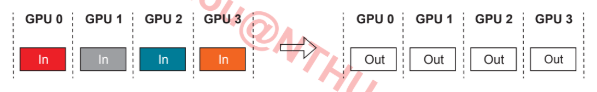
\includegraphics[width=0.75\linewidth]{FileAusiliari//Screenshots/Figure10-3.png}
    \caption{RCCL Allreduce 基本功能}
    \label{fig:RCCL_Allreduce_primitive}
\end{figure}

這次,我們不使用方便的\term{ncclCommInitAll},而是手動初始化通訊器。為此,我們首先需要獲取一個唯一ID,該ID用於綁定通訊器並允許\term{RCCL} 正確同步進程。為了告知\term{RCCL} 函式庫通訊器之間的關係,在創建時使用相同的唯一ID。因此,我們使用\term{MPI Broadcast} 基本功能將唯一ID從rank 0發送到所有其他rank。最後,在第25行,我們創建通訊器。

在執行緒或MPI模式下使用\term{RCCL} 通訊基本功能很簡單,因為不需要呼叫組API。當一個rank呼叫\term{ncclAllReduce} 時,\term{RCCL} 保持調用行程的進度並等待所有其他行程呼叫此API。當所有行程到達這一點時,\term{RCCL} 開始\term{AllReduce} 計算。

\begin{lstlisting}[language=C, caption={混合使用\term{MPI} 和\term{RCCL AllReduce}}, captionpos=t, label={lst:mpi_rccl_allreduce}]
int main(int argc, char* argv[]) {
   int size = 32 * 1024 * 1024;
   int myRank, nRanks = 0;
   
   // initializing MPI
   MPI_Init(&argc, &argv);
   MPI_Comm_rank(MPI_COMM_WORLD, &myRank);
   MPI_Comm_size(MPI_COMM_WORLD, &nRanks);
   
   ncclUniqueId id;
   ncclComm_t comm;
   float *sendbuff, *recvbuff;
   hipStream_t s;
   
   if (myRank == 0) ncclGetUniqueId(&id);
   MPI_Bcast((void*)&id, sizeof(id), MPI_BYTE, 0, MPI_COMM_WORLD);
   
   // Allocate buffers and create streams
   hipSetDevice(myRank);
   hipMalloc(&sendbuff, size * sizeof(float));
   hipMalloc(&recvbuff, size * sizeof(float));
   hipStreamCreate(&s);
   
   // Initializing RCCL
   ncclCommInitRank(&comm, nRanks, id, myRank);
   
   // communicating using RCCL
   ncclAllReduce((const void*)sendbuff, (void*)recvbuff, size,
                 ncclFloat, ncclSum, comm, s);
                 
   // Completing RCCL operation by synchronizing on the (HIP) stream
   hipStreamSynchronize(s);
   
   // Free device buffers
   hipFree(sendbuff);
   hipFree(recvbuff);
   
   // Finalizing NCCL
   ncclCommDestroy(comm);
   
   // Finalizing MPI
   MPI_Finalize();
   return 0;
}
\end{lstlisting}

透過這個範例,我們可以理解如何在多GPU計算環境中有效地運用\term{RCCL} 來處理特定的通訊模式。

\section{Conclusion}

在本章中,我們介紹了AMD \term{ROCm} 平台上不同的基於\term{HIP} 的多GPU程式設計選項。\term{ROCm} 和\term{HIP} 提供了高度的靈活性和豐富的功能,使程式設計師能夠實現多GPU效能擴展。本章首先解釋了如何使用\term{HIP} API來查詢GPU數量並選擇特定的GPU使用。接著我們介紹了三種多GPU程式設計方法(即基於串流、執行緒和\term{MPI} 的方法)。這些主要關注CPU如何向多個GPU分派任務。之後,我們認識到了GPU間通訊的需求,並介紹了兩種GPU-GPU通訊解決方案:一種使用記憶體複製API,另一種使用點對點記憶體存取。對於常見的多GPU通訊模式,\term{RCCL} 函式庫提供了一系列通訊基本功能,實現了高效能且易於使用的GPU-GPU通訊。